\subsection{Methodology}

\subsubsection{Project Outline}

The software was developed over the course of 3 months in February -- April
2014. After this project's inception planning was undertaken before any work on
the project started. A project plan was finished on 14th February 2014.

The key part of project plan was the Gantt chart seen in Figure
\ref{figure:gantt}. There are 6 stages: literature survey, experimental design
(specifying requirements), software development, software development
(including design), evaluation (subdivided in running simulation and analysing
results), writing up, and presentation (with software demonstration). The chart
also includes the two main submission deadlines and notes that university
spring holidays overlap with the project, when limited performance was
predicted.

It can be seen that most stages overlap to some extent in order to account for
parallel activities and uncertainty of the exact time needed for them. Some
buffer time is factored in as well: if the software development stage is
successful (i.e. the minimum requirements are implemented and accounted for in
the report) then any further features can be added as they are implemented.

\begin{figure}
  \begin{center}
    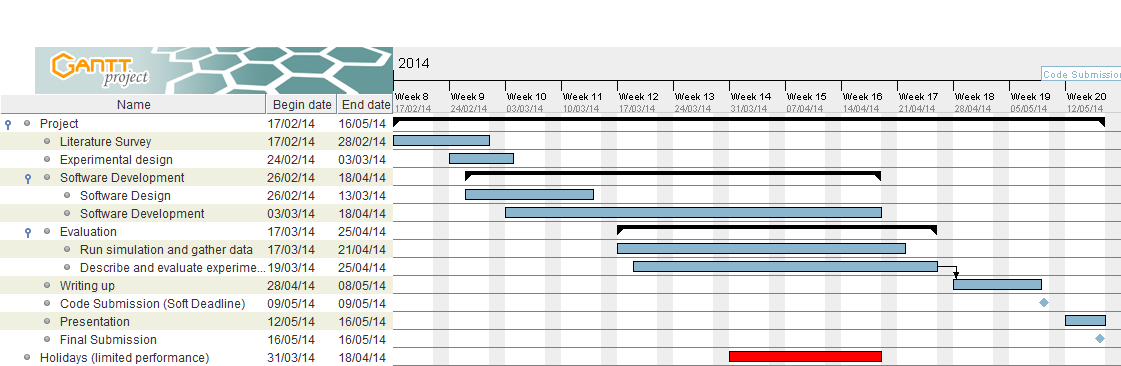
\includegraphics[width=\textwidth]{../figures/gantt}
    \caption{
      Project plan: Gantt activity chart
      \label{figure:gantt}
    }
  \end{center}
\end{figure}


\subsubsection{Processes}
\label{sec:design:processes}

At the project's inception it was agreed to have weekly meetings with the
supervisor to ensure that the project goes as planned and any issues can be
mitigated as soon as they arise. A risk assessment was done, identifying that
adhering to the timetable is critical to the project's success. It was also
noted that human or computer error causes risks of data damage, but can easily
be mitigated by using version control and backups (including cloud backup
storage).

The author has previous satisfactory experience of working with the Agile
software development philosophy (Scrum framework) and following the Test-Driven
Development (TDD) methodology. Particularly the software development aspects of
Scrum have a lot in common with a methodology called eXtreme Programming (XP)
\parencite{Copeland2001xp}. Agile philosophy, Scrum and XP are most useful for
teams working on larger projects \parencite(Cohn2010agile), so they will not be
discussed here any more.Still, TDD is one of the practices recommended by Scrum
(or XP) to improve software quality, and apart from most of Scrum it is aimed
at individual software developers \parencite{Beck2000xp, Cohn2010agile}. 

The TDD cycle goes as follows: automated tests are written first, followed by
writing program code which is finally refactored to improve quality -- this
results in a complete test coverage and a regression test suite which actually
enables safe refactoring. As an added benefit the automated test suite serves
as documentation for the code and helps explain developers' reasoning at the
time of writing software. \parencite{Beck2000xp}

Studies have found that TDD is better for code quality than traditional non-TDD
fashion: \textcite{Williams2003test} found that software produced in IBM
following TDD had 40\% less bugs, and \textcite{Bhat2006tdd} found a 50\%
increase in code quality in two different environments. However,
\textcite{Bhat2006tdd} also notes that TDD required 15\% more time upfront to
write tests. Finally, \textcite{Dhh2014tdd} warns about blindly following TDD
and not employing other tools and practices that could aid software
development.

Therefore it was chosen to follow TDD as closely as possible without
compromising other aspects of development. The implemented tests are discussed
in more detail in Section \ref{sec:implementation:testing} with actual examples
and discussion of how the author managed TDD.
